\documentclass[french]{extarticle}
\usepackage{fancyhdr}
\pagestyle{fancy}
\setcounter{secnumdepth}{4}
\setcounter{tocdepth}{4}

\usepackage{color}
\addtolength{\oddsidemargin}{-.8in}
\addtolength{\evensidemargin}{-.8in}
\addtolength{\textwidth}{1.6in}
\makeatletter

\makeatother
\usepackage{graphicx}
\usepackage[unicode=true,pdfusetitle,
 bookmarks=true,bookmarksnumbered=false,bookmarksopen=false,
 breaklinks=false,pdfborder={0 0 0},pdfborderstyle={},backref=false,colorlinks=true]
 {hyperref}
\hypersetup{
 linkcolor=blue,urlcolor=blue}

\makeatletter
\newcommand{\lyxrightaddress}[1]{
	\par {\raggedleft \begin{tabular}{l}\ignorespaces
	#1
	\end{tabular}
	\vspace{1.4em}
	\par}
}

\usepackage[svgnames]{xcolor}
\usepackage{svg}
\usepackage{rapport/lib/algorithmeUTF8}
\usepackage[utf8]{inputenc}

\usepackage{fancyhdr}
\lhead{Rapport projet Othello}
\chead{}
\rhead{}
\lfoot{ASI3 2019-2020}
\cfoot{Page \thepage}
\rfoot{\today}
\usepackage{fancyvrb}
\renewcommand{\headrulewidth}{0.4pt}
\renewcommand{\footrulewidth}{0.4pt}
\addtolength{\headheight}{\baselineskip}
\makeatother

\begin{document}
\rhead{
\includegraphics[height=1cm]{./sourcesIMAGES/Logo_INSARouen.png}}
\title{Rapport de Projet\\
	Projet Othello}
\author{MELO DA SILVA Alexis - MESBAH Zacharia\\
SAIVRES Jerôme - SI Ruixu}
\date{2019 - 2020}
\maketitle
\newpage
\tableofcontents
\newpage
\section{TADs}
\documentclass[]{article}
\usepackage{babel}
\usepackage[utf8]{inputenc}
\usepackage{algorithmeUTF8} 
\begin{document}

	\begin{tad}
		\tadNom{Couleur}
		\tadDependances{Chaine de caractères}
		\begin{tadOperations}{Couleur}
			\tadOperation{Couleur}{\tadUnParam{Chaine de caractères}}{\tadUnParam{Couleur}}
			\tadOperation{CouleurOpposée}{\tadUnParam{Couleur}}{\tadUnParam{Couleur}}
			
		\end{tadOperations}
		\begin{tadAxiomes}
			\tadAxiome{CouleurOpposée( CouleurOpposée( Couleur ))) = Couleur}
		\end{tadAxiomes}
	\end{tad}
	
	\begin{tad}
		\tadNom{Pion}
		\tadDependances{Couleur}
		\begin{tadOperations}{Pion}
			\tadOperation{Pion}{\tadUnParam{Couleur}}{\tadUnParam{Pion}}
			\tadOperation{ObtenirCouleur}{\tadUnParam{Pion}}{\tadUnParam{Couleur}}
			\tadOperation{InverserCouleur}{\tadUnParam{Pion}}{\tadUnParam{Pion}}
		\end{tadOperations}
		\begin{tadAxiomes}
			\tadAxiome{InverserCouleur(InverserCouleur(Pion(Couleur))) = Pion}
		\end{tadAxiomes}
	\end{tad}
	
	\begin{tad}
		\tadNom{Position}
		\tadDependances{Colonne,Ligne}
		\begin{tadOperations}{Position}
			\tadOperation{Position}{\tadUnParam{Colonne x Ligne}}{\tadUnParam{Position}}
			\tadOperation{FixerColonne}{\tadUnParam{Colonne}}{\tadUnParam{Position}}
			\tadOperation{FixerLigne}{\tadUnParam{Ligne}}{\tadUnParam{Position}}
			\tadOperation{ObtenirColonne}{\tadUnParam{Position}}{\tadUnParam{Colonne}}
			\tadOperation{ObtenirLigne}{\tadUnParam{Position}}{\tadUnParam{Ligne}}
		\end{tadOperations}
		\begin{tadAxiomes}
		\end{tadAxiomes}
	\end{tad}
	
	\begin{tad}
		\tadNom{Coup}
		\tadDependances{Position,Pion,Plateau}
		\begin{tadOperations}{Coup}
			\tadOperation{Coup}{\tadUnParam{Position x Pion}}{\tadUnParam{Coup}}
			\tadOperation{ObtenirPosition}{\tadUnParam{Coup}}{\tadUnParam{Position}}
			\tadOperation{ObtenirPion}{\tadUnParam{Coup}}{\tadUnParam{Pion}}
			\tadOperation{EstValideCoup}{\tadUnParam{Plateau}}{\tadUnParam{Booleen}}
		\end{tadOperations}
		\begin{tadAxiomes}
		\end{tadAxiomes}
	\end{tad}
	
	\begin{tad}
		\tadNom{Plateau}
		\tadDependances{Position,Coup,Plateau,Pion}
		\begin{tadOperations}{Plateau}
			\tadOperation{Plateau}{\tadUnParam{Naturel x Naturel}}{\tadUnParam{Plateau}}
			\tadOperation{JouerCoup}{\tadUnParam{Plateau x Coup}}{\tadUnParam{Plateau}}
			\tadOperation{ObtenirPion}{\tadUnParam{Plateau x Position}}{\tadUnParam{Pion}}
			\tadOperation{CaseVide}{\tadUnParam{Plateau x Position}}{\tadUnParam{Booleen}}
			\tadOperation{Remplacer}{\tadUnParam{Plateau x Position}}{\tadUnParam{Plateau}}
		\end{tadOperations}
		\begin{tadAxiomes}
			\tadAxiome{ObtenirPion(JouerCoup(Plateau,Coup(Position,Pion)), Position) = Pion}
			\tadAxiome{Remplacer(Remplacer(Plateau,Position),Position) = Plateau}
		\end{tadAxiomes}
	\end{tad}
	
	\begin{tad}
		\tadNom{Coups}
		\begin{tadOperations}{Coups}
			\tadOperation{Coups}{}{\tadUnParam{Ensemble<Coup>}}
			\tadOperation{AjouterCoup}{\tadUnParam{Coups x Coup}}{\tadUnParam{Coups}}
			\tadOperation{RetirerCoup}{\tadUnParam{Coups x Coup}}{\tadUnParam{Coups}}
			\tadOperation{NombreCoups}{\tadUnParam{Coups}}{\tadUnParam{Naturel}}
		\end{tadOperations}
		
	\end{tad}
	
\end{document}
\newpage
\section{Analyse descendante}
\begin{figure}[h]
  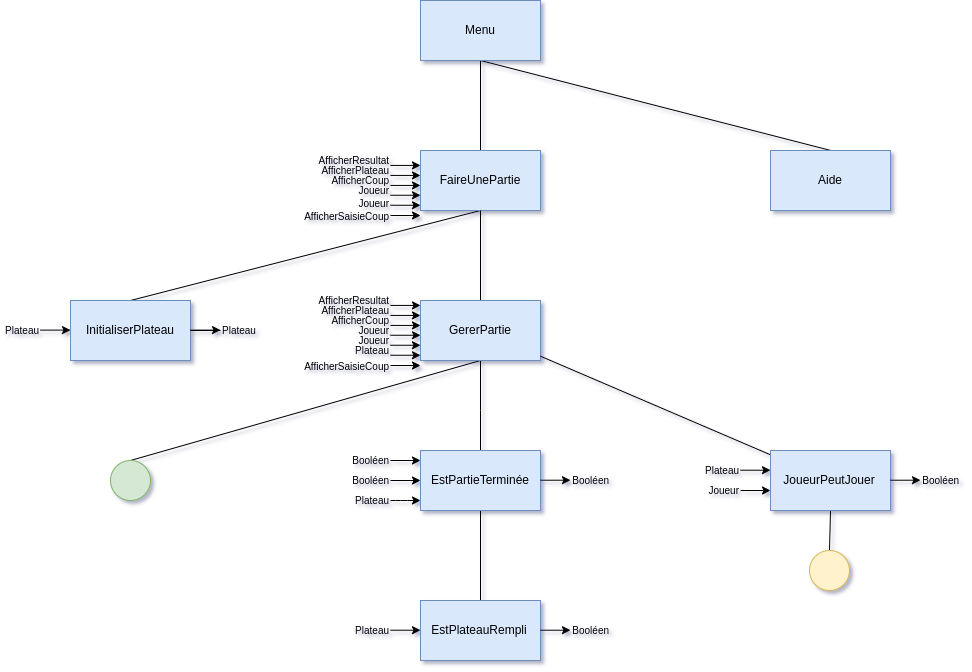
\includegraphics[width=18cm]{./sourcesIMAGES/analyse_main.png}
  \caption{Base principale de l'analyse descendante}
\end{figure}
\newpage
\begin{figure}[h]
  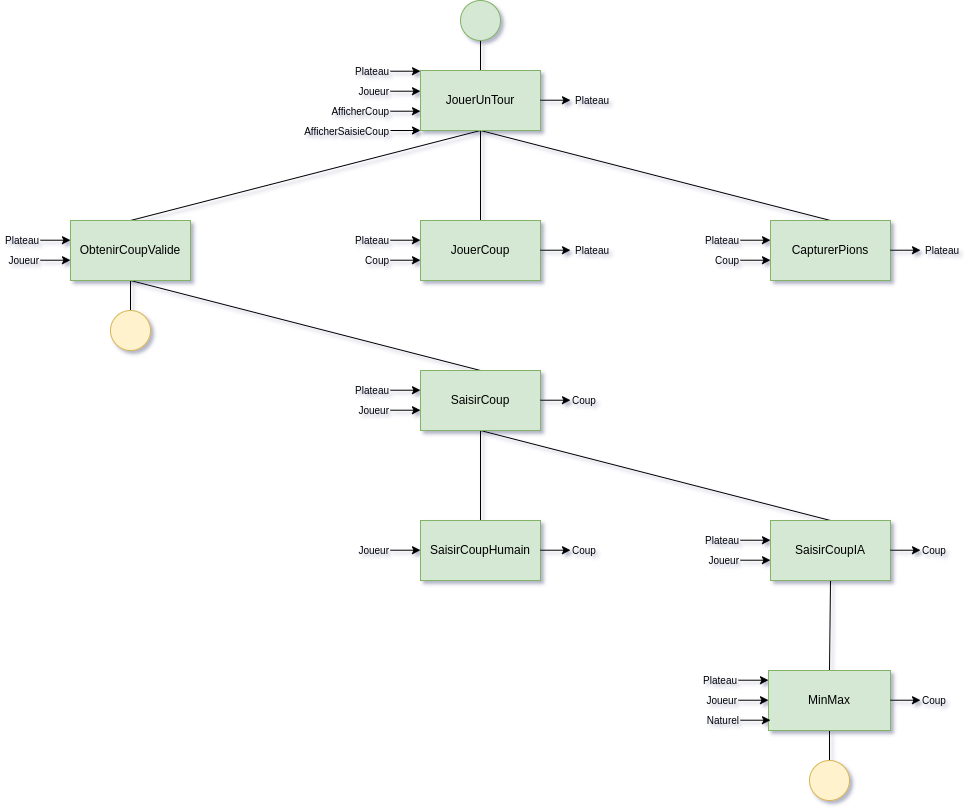
\includegraphics[width=18cm]{./sourcesIMAGES/analyse_jouerUnTour.png}
  \caption{Sous arbre de l'analyse descendante découlant de la méthode JouerUnTour}
\end{figure}
\begin{figure}[h]
  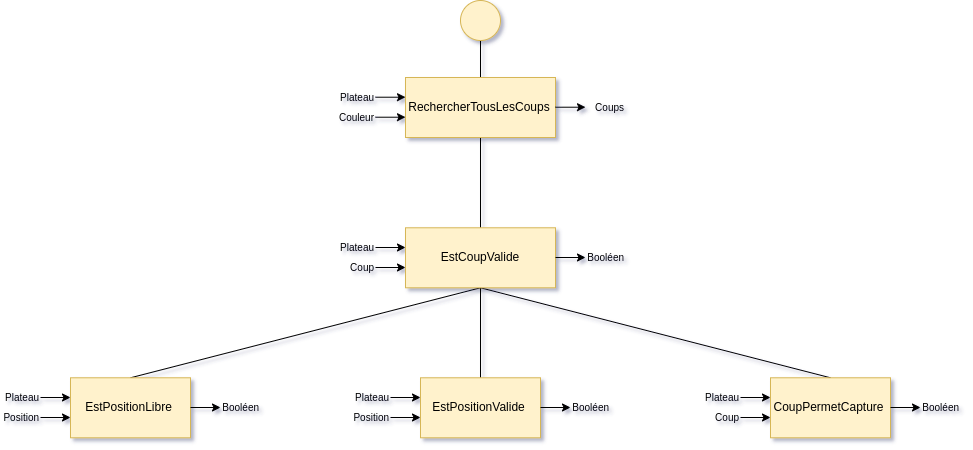
\includegraphics[width=18cm]{./sourcesIMAGES/analyse_chercherTousLesCoups.png}
  \caption{Sous arbre de l'analyse descendante découlant de la méthode RechercherTousLesCoups}
\end{figure}

\newpage
\section{Conception preliminaire}
   \subsection{TAD Couleur}
    \begin{algorithme}
    \signaturefonction{creerBlanc}{}{\textbf{Couleur}}
    \signaturefonction{creerNoir}{}{\textbf{Couleur}}
    \signaturefonction{creerNeutre}{}{\textbf{Couleur}}
    \signaturefonction{ObtenirCouleurOpposee}{couleur : Couleur}{\textbf{Couleur}}
    \signaturefonction{estNeutre}{}{\textbf{Couleur}}
    \signaturefonction{FixerCouleurOpposee}{couleur : Couleur, couleurOpposee : Couleur}{\textbf{Couleur}}
    \end{algorithme}
    \subsection{TAD Direction}
     \begin{algorithme}
    \signaturefonction{creerH}{}{\textbf{Direction}}
    \signaturefonction{creerHD}{}{\textbf{Direction}}
    \signaturefonction{creerD}{}{\textbf{Direction}}
    \signaturefonction{creerBD}{}{\textbf{Direction}}
    \signaturefonction{creerB}{}{\textbf{Direction}}
    \signaturefonction{creerBG}{}{\textbf{Direction}}
    \signaturefonction{creerG}{}{\textbf{Direction}}
    \signaturefonction{creerHG}{}{\textbf{Direction}}
    \signaturefonction{ObtenirDecalageColonne}{direction : Direction}{\textbf{-1},\textbf{0},\textbf{1}}
    \signaturefonction{ObtenirDecalageLigne}{direction : Direction}{\textbf{-1},\textbf{0},\textbf{1}}
    \end{algorithme}
    \subsection{TAD Etat}
     \begin{algorithme}
    \signaturefonction{creerTermine}{}{\textbf{Etat}}
    \signaturefonction{creerEnCours}{}{\textbf{Etat}}
    \signaturefonction{creerBloque}{}{\textbf{Etat}}
    \signaturefonction{EtatDeLaPartie}{plateauDeJeu : PLateau, joueurActuel : Couleur}{\textbf{Etat}}
    \end{algorithme}
    
    
\subsection{TAD Position}
\begin{algorithme}
	\signaturefonction{CreerPosition}{c : Colonne, l : Ligne}{Position}
	\signatureprocedure{AppliquerDirection}{\paramEntreeSortie unePostion : Position, \paramEntree uneDirection : Direction}
	\signaturefonction{FixerColonne}{c : Colonne, l : Ligne}{Position}
	\signaturefonction{FixerLigne}{c : Colonne}{Position}
	\signaturefonction{ObtenirColonne}{unePostion : Position}{Colonne}
	\signaturefonction{ObtenirLigne}{unePostion : Position}{Ligne}
	\signaturefonction{EstEgalPosition}{position1, position2 : Position}{\booleen}
\end{algorithme}


\subsection{TAD Coup}
\begin{algorithme}
	\signaturefonction{CreerCoup}{unePostion : Position, uneCouleur : Couleur}{Coup}
	\signaturefonction{ObtenirPosition}{unCoup : Coup}{Position}
	\signaturefonction{ObtenirCouleur}{unCoup : Coup}{Couleur}
	\signaturefonction{EstCoupValide}{unPlateau : Plateau}{\booleen}
	\signaturefonction{EstEgalCoup}{coup1, coup2 : Coup}{\booleen}
\end{algorithme}


\subsection{TAD Coups}
\begin{algorithme}
	\signaturefonction{CreerCoups}{}{Ensemble $<$Coup$>$} \\
	Nous prendrons pour la suite :  Coups = Ensemble $<$Coup$>$
	\signaturefonction{EstVide}{lesCoups : Coups}{\booleen}
	\signatureprocedure{AjouterCoup}{\paramEntreeSortie lesCoups : Coups, \paramEntree unCoup : Coup}
	\signatureprocedure{RetirerCoup}{\paramEntreeSortie lesCoups : Coups, \paramEntree unCoup : Coup}
	\signaturefonction{ObtenirCoup}{lesCoups : Coups}{Coup}
	\signaturefonction{ObtenirNombreDeCoups}{lesCoups : Coups}{\naturel}
	\signaturefonction{EstPresent}{lesCoups : Coups, unCoup : Coup}{\booleen}
\end{algorithme}


\subsection{TAD Plateau}
\begin{algorithme}
	\signaturefonction{CreerPlateau}{}{Plateau}
	\signatureprocedure{InitialiserPlateau}{\paramEntreeSortie unPlateau : Plateau}
	\signatureprocedure{JouerCoup}{\paramEntreeSortie unPlateau : Plateau, \paramEntree unCoup : Coup}
	\signaturefonction{ObtenirCouleurAvecPosition}{unPlateau : Plateau, unePosition : Position}{Couleur}
	\signaturefonction{EstPositionLibre}{unPlateau : Plateau, unePosition : Position}{\booleen}
	\signaturefonction{ObtenirTaille}{unPlateau : Plateau}{\naturel}
	\signaturefonction{EstRempli}{unPlateau : Plateau}{\booleen}
	\signaturefonction{CalculerPoints}{unPlateau : Plateau, uneCouleur : Couleur}{\naturel}
	\signaturefonction{EstPositionValide}{unPlateau : Plateau, unePosition : Position}{\booleen}
	\signatureprocedure{CapturerPions}{\paramEntreeSortie unPlateau : Plateau, \paramEntree unCoup : Coup}
	\signatureprocedure{CapturerPionsDansDirections}{\paramEntreeSortie unPlateau : Plateau, \paramEntree unCoup : Coup, \paramEntree uneDirection : Direction}
\end{algorithme}


\subsection{TAD Ligne}
\begin{algorithme}
	\signaturefonction{ObtenirLigneDepuisInt}{ligNum : 1 .. Taille}{Ligne}
	\signaturefonction{ObtenirNumeroLigne}{l : Ligne}{1 .. Taille}
	\signaturefonction{EstEgalLigne}{l1, l2 : Ligne}{\booleen}
\end{algorithme}


\subsection{TAD Colonne}
\begin{algorithme}
	\signaturefonction{ObtenirColonneDepuisInt}{colNum : 1 .. Taille}{Colonne}
	\signaturefonction{ObtenirColonneDepuisInt}{colChar : Char}{Colonne}
	\signaturefonction{ObtenirNumeroColonne}{c : Colonne}{1 .. Taille}
	\signaturefonction{EstEgalColonne}{c1, c2 : Colonne}{\booleen}
\end{algorithme}

\subsection{Analyse descendante bleue}	
	\begin{algorithme}
		\signaturefonction{FaireUnePartie}{AfficherResultat, AfficherPlateau, AfficherCoup, AfficherSaisieCoup : Fonction, j1, j2 : Joueur}{}
	\end{algorithme}
	\begin{algorithme}
		\signatureprocedure{InitialiserPlateau}{\paramEntreeSortie plateau : Plateau}
	\end{algorithme}
	\begin{algorithme}
		\signatureprocedure{GererPartie}{\paramEntree AfficherResultat, \paramEntree AfficherPlateau, \paramEntree AfficherCoup, \paramEntree AfficherSaisieCoup : Fonction, \paramEntree j1, \paramEntree j2 : Joueur, \paramEntreeSortie plateau : Plateau}
	\end{algorithme}
	\begin{algorithme}
		\signaturefonction{EstPartieTerminee}{plateau : Plateau, j1PeutJouer, j2PeutJouer : \booleen}{\booleen}
	\end{algorithme}
	\begin{algorithme}
		\signaturefonction{JoueurPeutJouer}{plateau : Plateau, joueur : Joueur}{\booleen}
	\end{algorithme}
	\begin{algorithme}
		\signaturefonction{EstRempli}{plateau : Plateau}{\booleen}
	\end{algorithme}
	
\subsection{Analyse descendante verte}	
	\begin{algorithme}
		\signatureprocedure{JouerUnTour}{\paramEntreeSortie plateau : Plateau, \paramEntree joueur : Joueur, \paramEntree AfficherCoup, \paramEntree AfficherSaisieCoup : Fonction}
	\end{algorithme}
	\begin{algorithme}
		\signatureprocedure{CapturerPions}{\paramEntreeSortie plateau : Plateau, \paramEntree coup : Coup}
	\end{algorithme}
	\begin{algorithme}
		\signatureprocedure{JouerCoup}{\paramEntreeSortie plateau : Plateau, \paramEntree coup : Coup}
	\end{algorithme}
	\begin{algorithme}
		\signaturefonction{ObtenirCoupValide}{plateau : Plateau, joueur : Joueur}{\textbf{Coup}}
	\end{algorithme}
	\begin{algorithme}
		\signaturefonction{SaisirCoup}{j : Joueur, plateau : Plateau}{\textbf{Coup}}
	\end{algorithme}
	\begin{algorithme}
		\signaturefonction{SaisirCoupHumain}{j : Joueur}{\textbf{Coup}}
	\end{algorithme}
	\begin{algorithme}
		\signaturefonction{SaisirCoupIA}{j : Joueur, plateau : Plateau}{\textbf{Coup}}
	\end{algorithme}
	\begin{algorithme}
		\signaturefonction{MinMax}{plateau : Plateau, joueurAMaximiser : Joueur, profondeur : \naturel}{\textbf{Coup}}
	\end{algorithme}

\subsection{Analyse descendante jaune}	
	\begin{algorithme}
		\signaturefonction{RechercherTousLesCoups}{plateauDeJeu : Plateau, couleurJoueurActuel : Couleur}{\textbf{Coups}}
	\end{algorithme}
	\begin{algorithme}
		\signaturefonction{EstCoupValide}{plateau : Plateau, coup : Coup}{\textbf{\booleen}}
	\end{algorithme}
	\begin{algorithme}
		\signaturefonction{EstPositionLibre}{plateau : Plateau, position : Position}{\textbf{\booleen}}
	\end{algorithme}
	\begin{algorithme}
		\signaturefonction{EstPositionValide}{plateau : Plateau, position : Position}{\textbf{\booleen}}
	\end{algorithme}
	\begin{algorithme}
		\signaturefonction{CoupPossibleDansUneDirectionQuelconque}{plateau : Plateau, coup : Coup}{\textbf{\booleen}}
	\end{algorithme}
	\begin{algorithme}
		\signaturefonction{CoupPossibleDansDirection}{plateau : Plateau, coup : Coup, direction : Direction}{\textbf{\booleen}}
	\end{algorithme}
\newpage
\section{Types}
\begin{algorithme}

	\begin{enregistrement}{Couleur}
		\champEnregistrement{nom}{Chaine de caractères}
		\champEnregistrement{hexa}{Chaine de caractères}
		\champEnregistrement{couleurOpposee}{Couleur}
		\champEnregistrement{symbole}{Caractère}
		\champEnregistrement{estNeutre}{\booleen}
	\end{enregistrement}
\\
	\begin{enregistrement}{Pion [DEPRECATED]}
		\champEnregistrement{couleur}{Couleur}
	\end{enregistrement}
\\
	\begin{enregistrement}{Position}
		\champEnregistrement{ligne}{Ligne}
		\champEnregistrement{colonne}{Colonne}
	\end{enregistrement}
\\

	\begin{enregistrement}{Coup}
		\champEnregistrement{couleur}{Couleur}
		\champEnregistrement{position}{Position}
	\end{enregistrement}
\\\\
	\textbf{Type} Plateau \textbf{=} Tableau[1...Taille][1...Taille] de Couleur
\\\\
	\textbf{Type} Coups \textbf{=} Ensemble$<$Coup$>$
\\\\
	\textbf{Type} Ligne \textbf{=} 1...Taille
\\\\
	\textbf{Type} Colonne \textbf{=} 1...Taille
\\\\
	\begin{enregistrement}{Direction}
		\champEnregistrement{decalageLigne}{\{-1,0,1\}}
		\champEnregistrement{decalageColonne}{\{-1,0,1\}}
	\end{enregistrement}
\\\\
	\textbf{Type} Etat \textbf{=} {\{EN COURS, BLOQUE, TERMINE\}}


\end{algorithme}

\newpage
\section{Conception détaillée}
\begin{algorithme}
	\small
	\procedure
	{Initialiser Plateau}
	{\paramEntreeSortie p : Plateau}
	{ObtenirTaille(p) : \naturelNonNul \\
	blanc, noir, neutre : Couleur}
	{
	\affecter{neutre}{creerNeutre()}
	\affecter{blanc}{creerBlanc()}
	\affecter{noir}{creerNoir()}
	\pour{i}{1}{ObtenirTaille(p)}{}{

		\pour{j}{1}{ObtenirTaille(p)}{}{

			\instruction{JouerCoup(plateau,Coup(neutre,Position(Ligne(i),Colonne(j))))}
		}
	}

	\instruction{JouerCoup(plateau,Coup(blanc,Position(Ligne(ObtenirTaille(p) div 2),Colonne(ObtenirTaille(p) div 2))))}

	\instruction{JouerCoup(plateau,Coup(blanc,Position(Ligne(ObtenirTaille(p) div 2 + 1),Colonne(ObtenirTaille(p) div 2 + 1))))}

	\instruction{JouerCoup(plateau,Coup(noir,Position(Ligne(ObtenirTaille(p) div 2),Colonne(ObtenirTaille(p) div 2 + 1))))}

	\instruction{JouerCoup(plateau,Coup(noir,Position(Ligne(ObtenirTaille(p) div 2 + 1),Colonne(ObtenirTaille(p) div 2))))}
	}
\end{algorithme}

\begin{algorithme}
	\small
	\fonction
	{FaireUnePartie}
	{joueur = Couleur, ProfondeurIA = Naturel}
	{}
	{plateau = Plateau}
	{
	\affecter{plateau}{InitialiserPlateau()}
	\tantque{non FinirLaPartie}{
		\affecter{plateau}{JouerUnTour(plateau, joueur, ProfondeurIA)}
		\affecter{joueur}{Inverser(joueur)}
	}
	}
\end{algorithme}
\begin{algorithme}
	\small
	\fonction
	{plateauRempli}
	{plateauDeJeu : Plateau}
	{\booleen}
	{i : 1 .. Longueur
	 j : 1 .. Largeur
	 estRempli : \booleen}
	{
	\affecter{i}{1}
	\affecter{j}{1}
	\affecter{estRempli}{Vrai}
	\tantque{(i <= Longueur et estRempli)}{
		\tantque{(j <= Largeur et estRempli)}{
			\affecter{estRempli}{non(caseVide(plateauDeJeu,Position(i,j)))}
			\affecter{j}{j + 1}
		}
		\affecter{i}{i + 1}
	}
	\retourner{estRempli}
	}
\end{algorithme}
\begin{algorithme}
	\small
	\fonction
	{etatDelaPartie}
	{plateauDeJeu : Plateau, joueurActuel : Couleur}
	{Etat}
	{}
	{
	\sialorssinon {plateauRempli(plateauDeJeu)}
		{\retourner{(terminé)}}
	{	
	\sialorssinon {coupValideExiste(joueurActuel,plateauDeJeu)}
		{\retourner{(enCours)}}
		{\retourner{(bloqué)}}
	}
	}
\end{algorithme}
\begin{algorithme}
	\small
	\fonction
	{coupValideExiste}
	{plateauDeJeu : Plateau, joueurActuel : Couleur}
	{\booleen}
	{coupsValides : Coups}
	{
	\affecter{coupsValides}{chercherTousLesCoups(joueurActuel, plateauDeJeu)}
	\sialorssinon {estVide(coupsValides)}
		{\retourner{(Faux)}}
		{\retourner{(Vrai)}}
	}
\end{algorithme}
\begin{algorithme}
	\small
	\procedure
	{JouerUnTour}
	{\paramEntreeSortie plateau : Plateau, \paramEntree joueur : Joueur, \paramEntree AfficherCoup, \paramEntree AfficherSaisieCoup : Fonction}
	{coupAJouer : Coup}
	{
	\instruction{AfficherSaisieCoup(joueur)}
	\affecter{coupAJouer}{ObtenirCoupValide(plateau, joueur)}
	\instruction{JouerCoup(plateau, coupAJouer)}
	\instruction{CapturerPions(plateau, coupAJouer)}
	\sialors{EstIA(joueur)}
		{\instruction{AfficherCoup(coupAJouer)}}
	}
\end{algorithme}
\begin{algorithme}
	\small
	\fonction
	{rechercherTousLesCoups}
	{plateauDeJeu : Plateau, joueurActuel : Couleur}
	{Coups}
	{lesCoups : Coups \\
	i : 1 .. Taille \\
	j : 1 .. Taille}
	{
	\pour{i}{1}{Taille}{}{
		\pour{j}{1}{Taille}{}{
			\sialors {rechercherUnCoup (plateauDeJeu, joueurActuel, Position(i,j))}
				{\instruction{ajouterCoup (lesCoups, coup(Position(i,j), joueurActuel)}}
		}
	}
	\retourner{(lesCoups)}
	}
\end{algorithme}

\vspace*{2cm}

\begin{algorithme}
	\small
	\fonction
	{rechercherUnCoup}
	{plateauDeJeu : Plateau, joueurActuel : Couleur, positionDuCoup : Position}
	{\booleen}
	{}
	{
	\sialorssinon {EstPositionVide (plateauDeJeu, positionDuCoup)}
			{\retourner{parcourirLesDirections (unPlateauDeJeu, positionDuCoup, joueurActuel)}}
			{\retourner{(Faux)}}		
	}
\end{algorithme}

\vspace*{2cm}

\begin{algorithme}
	\small
	\fonction
	{parcourirLesDirections}
	{unPlateauDeJeu : Plateau, positionDuCoup : Position, joueurActuel: Couleur}
	{\booleen}
	{}
	{
	\retourner{parcourirUneDirection (unPlateauDeJeu, positionDuCoup, HG, joueurActuel)\\
	ou (parcourirUneDirection (unPlateauDeJeu, positionDuCoup, H, joueurActuel)\\
	ou (parcourirUneDirection (unPlateauDeJeu, positionDuCoup, HD, joueurActuel)\\
	ou (parcourirUneDirection (unPlateauDeJeu, positionDuCoup, D, joueurActuel)\\
	ou (parcourirUneDirection (unPlateauDeJeu, positionDuCoup, BD, joueurActuel)\\
	ou (parcourirUneDirection (unPlateauDeJeu, positionDuCoup, B, joueurActuel)\\
	ou (parcourirUneDirection (unPlateauDeJeu, positionDuCoup, BG, joueurActuel)\\
	ou (parcourirUneDirection (unPlateauDeJeu, positionDuCoup, G, joueurActuel)}
	}
\end{algorithme}

\vspace*{2cm}

\begin{algorithme}
	\small
	\fonction
	{parcourirUneDirection}
	{unPlateauDeJeu : Plateau, positionDuCoup : Position, uneDirection : Direction, joueurActuel : Couleur}
	{\booleen}
	{ligneEnCours, directionValide : \booleen \\
	i : 1 .. Taille\\
	j : 1 .. Taille}
	{
	\affecter{i}{obtenirNumeroLigne (positionDuCoup)}
	\affecter{j}{obtenirNumeroColonne (positionDuCoup)}
	\affecter{ligneEnCours}{Faux}
	\affecter{directionValide}{Faux}
	\instruction{appliquerDirection (positionDuCoup, uneDirection)}
	\sialors{obtenirCouleur (unPlateauDeJeu, positionDuCoup) $\neq$ joueurActuel}{
		\affecter{ligneEnCours}{Vrai}
		\tantque{(non directionValide et ligneEnCours)}{
			\instruction{appliquerDirection (positionDuCoup, uneDirection)}
			\sialorssinon {EstPositionVide (plateauDeJeu, positionDuCoup)}
				{\affecter{ligneEnCours}{Faux}}
				{\sialors{obtenirCouleur (unPlateauDeJeu, positionDuCoup) = joueurActuel}
					{\affecter{directionValide}{Vrai}}}
		}
	}
	\retourner{(directionValide)}
	}
\end{algorithme}
\begin{algorithme}
	\small
	\fonction
	{ObtenirCoupJoueur}
	{c : Couleur}
	{Coup}
	{ligne : Ligne, colonne : Colonne}
	{
	\affecter{ligne}{Ligne(input())}
	\affecter{colonne}{Colonne(input())}
	
	\retourner{Coup(Pion(c), Position(ligne, colonne))}
	}
\end{algorithme}
\begin{algorithme}
	\small
	\fonction
	{CalculPoint}
	{plateau : Plateau, couleur : Couleur}
	{Naturel}	
	{points : Naturel
	i, j : Naturel Non Nul}
	{
	\pour{i}{1}{8}{}{
		\pour{j}{1}{8}{}{
			\sialors	{couleur = ObtenirCouleur(ObtenirPion(plateau, positionposition(i, j)}{
				\affecter{points}{points + 1}			
			}
		}
	}
	}
\end{algorithme}
\end{document}
